\section{Experiments}

In the next section, we present methods which we believe are optimal for the proper implementation of an MVP. We will summarize the most significant experiments we ran and hint at the results produced. However, we will discuss the quantitative and qualitative results in the results section of this paper.


\subsection{Face and emotion detection}

We used a traditional Haar-Cascade classifier to detect faces within the camera's frame. To test the accuracy and detection rate, we recorded five short videos, 400 frames in length each. We used these frames to test the time it took the classifier to produce a result.

The features we are looking for in our frames are both faces and eye features for two reasons. We want to keep a person within the camera's frame, and we also want to pass a cropped photo of the person to the emotion detector, which performs best when both eyes are visible. 

Regarding emotion detection, we used the CNN provided by Octavio Arriaga \cite{DBLP:journals/corr/abs-1710-07557}. In their publication, they report 66\% accuracy on the FER dataset on their "sequential fully-CNN."

When training this on FERPlus, we simplified the number of classes to 5 as we found that the robot's behavior was too erratic with more classes. Our chosen emotions are happiness, surprise, fear, sadness, and anger.


We measure the performance of our face and emotion detection algorithms by how much time it takes for them to produce a result, as each passing frame affects the quality of the final product.

\subsection{Style Transfer}


We started by taking Karras' team StyleGAN2 network description and adapting it to run on the Raspberry Pi 4s hardware. 


The purpose of using Karras' model was to minimize the requirements for inference of a trained model following their architecture. Our logic was that by minimizing the model's footprint, the inference would be fast enough to complete in real-time for our robot. In our early testing, reducing the input images to even below 100 x 100 px produced a model with an inference time of around 30 seconds per frame on the Raspberry Pi hardware. We decided that the optimizations required to make this model work at a more reasonable speed were outside of our expertise, as we quickly realized that it required a deeper understanding of the Raspberry Pi's hardware to make use of platform-specific instructions. 

We moved on to implementing Justin Johnson's solution on our platform. Jhonson's original publication used Lua with Torch packages to implement a feedforward neural network to improve the speed of the original Gatys et al. paper's results. This implementation takes around 50 milliseconds per frame on a 1200 x 630-pixel image, which seems promising. 

Jhonson's team initially implemented their network for Lua with Luarocks and Torch packages. We translated Jhonson's network architecture to Python with Pytorch 1.9 as close to the original architecture as possible. We noticed that, as Jhonson points out in his publication, changing instance normalization in place of batch normalization has a very sizeable impact on speed performance at the cost of very minimal visual performance. We call this network "PiStyle", as it allowed us to implement style transfer in near real-time.


Using the PiStyle network for our implementation, we split the model's functioning into two parts: low-resolution mode and high-resolution mode. When the robot shows the style transfer "live" to the user, we use a low-resolution pre-trained model. This model outputs images at a 125 x 125-pixel resolution, which are upscaled using bicubic interpolation to our display's native resolution of 1024 x 600 pixels. The network switches to the high-resolution mode whenever the user requests an image. This mode is slower than the low-resolution mode but can output images at a 1024 x 600-pixel resolution. These images are then upscaled using bicubic interpolation to 2560x1440 pixels and saved.

\subsection{Providing images for the user}

With all of our methods implemented, we need a way to get images to the user. The Telegram Bot API provides us with a simple and effective way to manage a user's data, as we can design it to only ever work with the user that has physical access to the bot. 

We implemented the necessary API calls to store the user's chat ID, which is needed to send messages through the Telegram API, and the API calls that send photos as messages to the user. Through the bot's interface on their Telegram app, they can choose any combination of photos they want to receive: original image, low-resolution style transfer, or high-resolution style transfer.

If the user does not want to use the Telegram bot, we save all images to an output folder accessible through the Raspberry Pi's storage card.


\subsection{Robot state diagram: how it comes together}

\begin{figure}[ht]
  \centering
  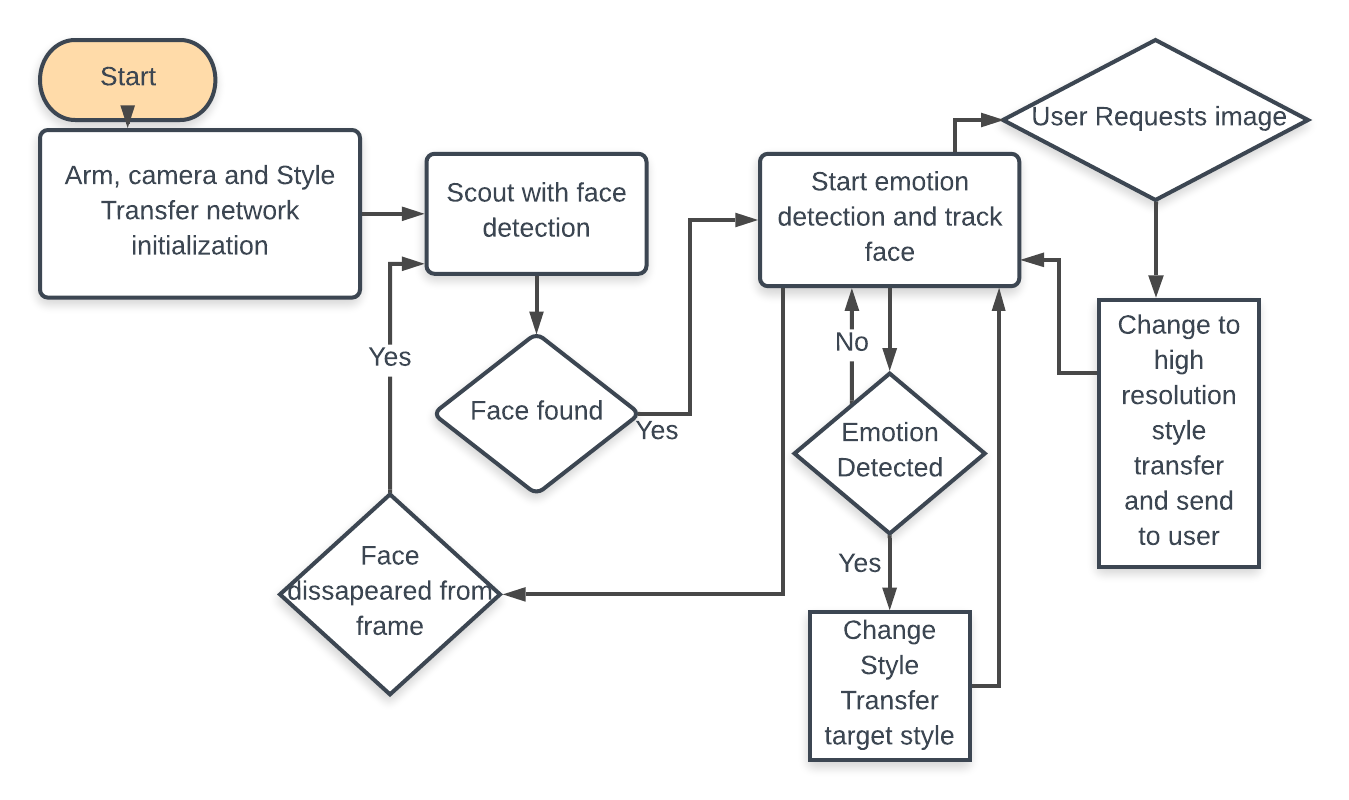
\includegraphics[width=\textwidth]{resources/state_machine.png}
  \caption{Robot state machine diagram.}\label{fig:state_machine}
\end{figure}

With all of our methods in place and working correctly, the only thing missing is the logic that connects them to form a product. In fig. \ref{fig:state_machine} you will find the state machine that describes our implementation of the robot's operating process. 




We tried to keep the diagram simple for clarity, so it requires a few clarifications.

If we follow an execution where a user starts the robot, walks into the field of view of the camera, and requests an image, these are the more in-depth descriptions of what each part of the process does:

\begin{enumerate}
  \item \textbf{User powers the robot on:} A script starts when the Raspberry Pi turns on, switching to the python virtual environment that contains all the necessary libraries for our scripts to work. The camera feed is started. The neural network for style transfer is initialized in low-resolution mode with a default style transfer, and its output is routed to the HDMI display attached to the robot. The arm initializes the position of the servomotors on fixed coordinates, pointing the camera towards the front of the robot.   
  \item \textbf{Robot searches for faces:} The arm starts panning around its horizontal field of view in 10º degree increments until it reaches its movement limit to one side and starts panning on the same 10º degree increments until it reaches the other side. Each time the arm completes a 10º movement, it captures an image frame and runs face detection on it. If there is no face found, it starts the next movement.
  \item \textbf{When a face is found, recognize emotion and perform live style transfer:} The face is cropped and fed into our emotion recognition script. The result of the emotion recognition engine is saved on a circular buffer of 5 frames, and the script outputs the average of these five results. This average is used to select one of 5 different styles for the style transfer algorithm. Suppose there is a change in emotion from the previously set style. In that case, the neural network is reinitialized with the corresponding style's pre-trained model (2-5 second overhead, depending on the source and target model).
  \item \textbf{Whenever the user requests it, provide them with a style transferred image file:} When the user uses the "capture" button, the last full-sized frame on the image is saved, along with its corresponding low-resolution style transfer. The camera feed is ignored throughout the following process. The full-sized frame is then fed to the high-resolution style transfer network. Then, the output is upscaled to 2560 x 1440 pixels using bicubic interpolation. All three files (original photo, low-resolution style transfer, high-resolution style transfer) are sent through the telegram bot to the user. After the robot sends the image, the user can cycle through the next high-resolution model for style, transferring the same original photo or going back to live-view, which reactivates the low-resolution style transfer mode.
  \item \textbf{Whenever the face is lost, go back to state 2.}
  \item \textbf{At any point:} The user can use a keypress for cycling through the available pre-trained models for the style transfer. If the user cycles to the next model, emotion recognition and style context switching are put on hold until they start it again.
\end{enumerate}